\section{Fachliche Grundlagen}


\subsection{Begriffserklärung}
Die Begriffe Anreiz, Motiv und Motivation werden im Alltag oft synonym verwendet. Zur Förderung des Verständnisses dieser Arbeit, werden im Folgenden diese Begriffe bestimmt und gegeneinander abgegrenzt. \citep[S. 19]{Nowka.2013}

\subsubsection{Motiv}
Ein Motiv ist die Erwartungshaltung, die einer Handlung zugrunde liegt. Somit kann das gesamte menschliche Verhalten als Motiv-gesteuert angesehen werden. Die Definition und Bewertung der jeweiligen Motive erfolgt individuell und subjektiv. Zusätzlich können Motive durch Umweltreize sowohl verstärkt wie vermindert werden. \citep[S. 19f]{Nowka.2013}

Desweiteren kann zwischen primären und sekundären Motiven unterschieden werden. Erstere werden durch physiologische Vorgänge im Organismus hervorgerufen, z.B. Hunger und Durst. Sekundäre Motive hingegen sind von der Umwelt erlernt, z.B. das Verdienen von Geld. \citep{Jung.2011}


\paragraph{Leistungsmotiv}
Das Motiv der Leistung das bis heute am meisten untersuchte Motiv. Es ist das Streben nach Exzellenz, die Suche nach der Herausforderung, die eigenen Fähigkeiten unter Beweis zu stellen. Vorraussetzung dafür ist immer eine Vergleichbarkeit. Entweder aus eigener Erfahrung, mit der Leistung Anderer oder allgemein anerkannter Gütestandards. Der Antrieb zur Leistung geht dabei von der Person selbst aus. Die zugrunde liegende Definition, was Leistung ist, kann sich dabei je nach kultureller und sozialer Zugehörigkeit unterscheiden. \citep[S. 145f]{Brunstein.2010}

\paragraph{Soziale Bindung: Anschlussmotiv und Intimitätsmotiv}
Den großteil seines Lebens verbringt der Mensch in Gesellschaft Anderer. Die Interaktion reicht dabei von beziehungslosem Miteinander über anonyme Konkurrenz bis hin zu aggressivem Gegeneinander. Die Voraussetzung zur zwischenmenschlichen Kommunikation ist dem Menschen dabei wie allen Säugetieren angeboren. Maßgeblichen Einfluss auf die Art der Kommunikation haben Emotionen. Sie wirken als Signale des Emotionsausdrucks und des Motivationszustandes einer Person. Ihr subjektives Erleben bildet in der Summe den aktuellen Motivationszustand einer Person. Zur Äußerung kommt dies in vielfältiger Form verbaler und nonverbaler Kommunikationsformen wie Gestik, Mimik, Stimmführung, Körperhaltung und Distanzveränderungen zu seinem Gegenüber.
Das Intimitätsmotiv entspricht umgangssprachlich der \glqq Liebe\grqq. Das Ziel ist die Schaffung und Erhaltung einer eng vertrauten Beziehung, sich gegenseitig austauschender Zweisamkeit.
Es gibt aber auch ein große Menge sozialer Interaktion, die nicht dem Anschlussmotiv angerechnet werden kann. Dazu zählen zum Beispiel das Messen mit Anderen, das Beherrschen anderer Menschen oder auch das umgangssprachliche “prahlen” vor Anderen. \citep[S. 193f]{Sokolowski.2010}

\paragraph{Machtmotiv}
Schon immer wurde versucht, die Macht in ihrer vielfältigen Form und ungleichen Verteilung zu Erklären, Rechtzufertigen oder Herauszufordern. Selbst bei nichtmeschlichen Primaten spielen Macht und Dominanz eine zentrale Rolle. Jedem Sozialgebilde jeglicher Form liegt eine differenzierende Verteilung der Macht zugrunde. Es scheint, dass es keines gibt, welches ohne diese dauerhaft überlebensfähig wäre. \citep[S. 211]{Schmalt.2010}

Der motivationspsychologische Ansatz beschreibt Macht als einen Austauschprozess zwischen verschiedenen Individuen. Die Individualebene betrachtet dabei die Motive, der Austauschprozess die Verhaltens- und Situativkomponente. \citep[S. 211f]{Schmalt.2010}

\subsubsection{Motivation}
Gabler beschreibt die Motivation als den \glqq Zustand einer Person, der sie dazu veranlasst, eine bestimmte Handlungsalternative auszuwählen, um ein bestimmtes Ergebnis zu erreichen und der dafür sorgt, dass diese Person ihr Verhalten hinsichtlich Richtung und Intensität beibehält\grqq. \citep{GablerMotivation.2014}

Drumm versteht \glqq unter Motivation (...) ein[en] geistig-seelische[n] Antrieb zur Steuerung und zum Vollzug des Handelns und Verhaltens \grqq. \citep[S. 384]{Drumm.2008}

Bei den genannten Defintionen lässt sich entnehmen, dass die Motivation maßgeblich eine Handlung vorantreibt. 

Nach Haubruck wird unter Motivation \glqq im Unternehmenskontext (...) in der Regel die Erhöhung und Förderung, teilweise auch die Aufrechterhaltung der Leistungsbereitschaft verstanden.\grqq \citep[S. 109]{Haubrock.2009}

\paragraph{Intrinsische Motivation}
Befriedigt die Tätigkeit als solche jemanden, empfindet er Spaß und Freude bei der Ausführung dieser, wird von intrinsischer Motivation gesprochen. Es ist der innere Drang etwas zu tun. \citep[S. 40f]{Nowka.2013} 

Der Flow-Effekt ist ein Zustand, bei welchem \glqq […] es sich um das selbstreflexionsfreie, gänzliche Aufgehen in einer glatt laufenden Tätigkeit [handelt], bei der man trotz voller Kapazitätsauslastung das Gefühl hat, den Geschehensablauf noch gut unter Kontrolle zu haben\grqq. \citep[S. 380]{Rheinberg.2010} 
Das selbstreflexionsfreie Arbeiten kommt dabei u.A. durch Vergessen der Zeit und Ausblendung aller persönlichen Sorgen zum Vorschein. 

\paragraph{Extrinsische Motivation}
Im Gegensatz zur intrinsischen Motivation steht bei der Extrinsischen nicht die Handlung an sich im Vordergrund, sondern die mögliche Belohung bzw. nicht-Bestrafung. Das Handeln basiert auf sekundären Motiven. So bedarf es eines, wie auch immer gearteten, von außen gesetzten Anreizes, zur Durchführung der Handlung bzw. Tätigkeit. \citep[S. 41f]{Nowka.2013}

\subsubsection{Anreiz}
\glqq Alles was Situationen an Positivem oder Negativem einem Individuum verheißen oder andeuten, wird als »Anreiz« bezeichnet, der einen »Aufforderungscharakter« zu einem entsprechenden Handeln hat. Dabei können Anreize an die Handlungstätigkeit selbst, das Handlungsergebnis und verschiedene Arten von Handlungsergebnisfolgen geknüpft sein.\grqq \citep[S. 5]{Heckhausen.2010b}
\citet[S. 106]{Beckmann.2010} ergänzen den Individualcharakter der Definition von \citet[S. 106]{Heckhausen.2010b} um die subjektive und affektive Bewertung der Sachverhalte. Mit der Verknüpfung eines Objekts mit einem Affekt ist es möglich, dass für ein Individuum ein Reiz Anreizcharakter erlangt. Starke Beeinflussung erfährt ein Anreiz durch organismische Zustände. Diese können seine Wirkung erhöhen oder senken. Dies konnte auch durch die neuropsychologische Forschung bestätigt werden. \citep[S. 106f]{Heckhausen.2010b}

\subsection{Motivationstheorien}
Die Motivationstheorien versuchen, den Zusammenhang von Motivation und menschlichem Verhalten zu beschreiben. Aus der Erkenntnis, dass die Motivation eines Mitarbeiters maßgeblich seine Leistung beeinflusst, haben sich drei wesentliche Theorien entwickelt:

- Inhaltstheorien beschäftigen sich mit \glqq der Art, Inhalt und Wirkung der Bedürfnisse von Individuen\grqq. \citep[S. 391]{Drumm.2008}

- Prozesstheorien betrachten den Prozess der Motivation losgelöst von Bedürfnisinhalten. \citep[S. 391]{Drumm.2008}

\subsubsection{Inhaltstheorien}
\paragraph{Die Zwei-Faktoren-Theorie von Frederick Herzberg}
Nach Herzberg unterteilen sich die Grundbedürfnisse eines Menschen in Hygienebedürfnisse und  Motivationsbedürfnisse.

Erstere führen bei Nichterfüllung zu Unzufriedenheit und werden daher als Selbstverständlichkeit angesehen. Sie führen bei Erfüllung jedoch nicht zu Zufriedenheit. Als Beispiele seien hier die Sicherheit des Arbeitsplatzes sowie eine angemessene Bezahlung genannt. \citep[S. 26]{Nowka.2013}

Die Erfüllung von Motivationsbedürfnissen hingegen führt zu Zufriedenheit. Herzberg bezeichnet diese als direkt auf die Tätigkeit bezogene Faktoren wie Anerkennung und Verantwortung. Er zielt damit auf die intrinsischen Arbeitsbedürfnisse eines Mitarbeiters ab. \citep[S. 26f]{Nowka.2013}

Kritik an Herzbergs Theorien bezieht sich vor allem auf die situative Abhängkeit der Motivatorien und Frustratoren sowie fehlende soziokulturelle Einflüsse. \citep[S. 396]{Drumm.2008}

\paragraph{Die Motivationstheorie von David C. McClelland}
McClelland setzt das Machtmotiv in das Zentrum seiner Theorie. Danach muss ein Vorgesetzter seinen Mitarbeitern das Gefühl eigener Macht vermitteln, ohne jedoch den Anschein der Unterwerfung zu erwecken. Grundvoraussetzung dafür ist, dass Autonomie und Verantwortung für das eigene Handeln bei jedem Mitarbeiter als äußere Bedingung gegeben sind. 
Zur Ausübung des Machtmotivs stellt McClelland drei lernbare Formen dar. Sie unterscheiden sich im Maß der Eigenverantwortung, welche den Mitarbeitern übertragen wird. Die einfachste Form ist die Persönliche Herrschaft der Führungskraft, gefolgt von einer uneigennützigen Machtausübung bis hin zur selbstlosen Führerschaft. \citep[S. 396ff]{Drumm.2008}

Kritisiert an McClellands Theorie wird vor allem der singuläre Fokus auf das Machtmotiv sowie das fehlende Zeitverhalten. Zugute zuhalten ist McClelland hingegen die zumindest teilweise Legitimation von Konzepten partizipativer Führung. \citep[S. 398]{Drumm.2008}

\subsubsection{Prozesstheorien}
\paragraph{Die VIE-Theorie von Vroom}
Die VIE-Theorie basiert auf den drei Variablen Valenz, Instrumentalität und Erwartung. Eine ihrer Kernaussagen ist es, dass Mitarbeiter zur Arbeit motiviert sind, wenn sie darin einen Weg sehen, ihre persönlichen Ziele zu erreichen. \citep[S. 30]{Nowka.2013}
 
Vroom konzentriert sich dabei auf den Prozessablauf. Die Valenz steht dabei für die \glqq […] persönlich empfundene Bedeutung des Handlungsergebnisses\grqq. \citep[S. 31]{Nowka.2013} Die Auslegung ist Situationsabhängig und kann sich mit der Zeit ändern. Die Instrumentalität entspricht der Tauglichkeit einer Handlung zur Zielerreichung. Die Erwartung lässt sich in Handlungs-Ergebnis-Erwartung und Ergebnis-Folge-Erwartung unterteilen.
Erstere beschreibt die subjektive Wahrscheinlichkeit der Zielerreichung einer Handlung unter Berücksichtigung weiterer Faktoren wie der individuellen Qualifikation und dem Grad der dafür notwendigen Anstrengung.
Letztere steht für die subjektive Wahrscheinlichkeit, die erwartete Belohnung tatsächlich zu erhalten. \citep[S. 31]{Nowka.2013}
 
Die Motivation entspricht dem Produkt aller drei Variablen. Das bedeutet aber auch, wenn eine der Variablen null ist, so ist die Motivation gleich null. \citep[S. 31]{Nowka.2013}
 
Kritik an der VIE-Theorie gibt es an der Prämisse, dass allgemein die Nutzenmaximierung als Ziel jedes Individuums unterstellt wird. \citep[S. 401]{Drumm.2008}

\subsection{Anreizsysteme}
Ein Anreizsystem besteht aus mehreren Anreizen im Wirkungsverbund mit dem Ziel, erwünschte Verhaltensweisen herbeizuführen und unerwünschte Verhaltensweisen zu unterdrücken. Aufgabe eines Anreizsystems ist es, anstatt mit explizit ausformulierten Verhaltensanweisungen, mit Zielvorgaben das gewünschte Verhalten implizit zu fördern bzw. unerwünschtes zu unterbinden. Zur Vereinfachung greifen Anreizsysteme meist nur wenige als typisch empfundene Bedürfnisse auf. Voraussetzung dafür sind zumindest begrenzte Entscheidungs- und Verhaltensfreiheiten der darin eingebundenen Individuen. Weitergehende Definitionen eines Anreizsystems im Unternehmenskontext umfassen auch Parameter wie Arbeitsbedingungen, Unternehmensimage sowie das Führungssystem des Unternehmens. \citep[S. 458]{Drumm.2008}

\subsection{Neurobiologische Grundlagen}
Im Verlauf dieses Abschnitts werden die für diese Arbeit relevante Teile des Gehirns und deren Zuständigkeiten dargestellt. Aufgrund der sehr komplexen Thematik werden die Sachverhalte hier nur in einer sehr vereinfachten Form beschrieben. 

\subsubsection{Das Gehirn}
Das Gehirn und das Rückenmark bilden zusammen das Zentralnervensystem des Menschen. Beide Teile sind \glqq sowohl funktionell als auch anatomisch untrennbar\grqq miteinander verbunden. \citep[S. 105]{Kirschbaum.2008} Im Durchschnitt wiegt das menschliche Gehirn 1500g und umfasst nach Schätzungen  ca. 100 Milliarden Nervenzellen die durch ca. 100 Billionen Synapsen miteinander verbunden sind. \citep{Weber.2011}

Das Gehirn besteht im Wesentlichen aus fünf Teilen, dem Groß- oder Endhirn, dem Hinterhirn (Kleinhirn), dem Zwischenhirn, dem Mittelhirn und dem Nachhirn (verlängertes Rückenmark). \citep{Schaefers.2014} Abbildung 1 zeigt den schematischen Aufbau des menschlichen Gehirns.

\begin{figure}[!h]
\centering
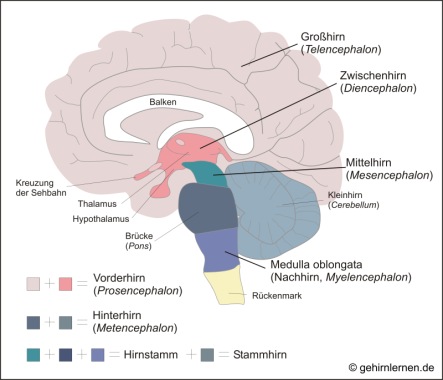
\includegraphics[width=0.8\linewidth]{grafiken/abb1.png}
\caption{Schematische Gliederung des Gehirns \\ Quelle: \cite{Schaefers.2014}}
\label{fig:Gehirn1}
\end{figure}

\begin{table}[!h]
\caption{Zuordnungen von Gehirnstrukturen zu Funktionen}
\label{Tabelle1}
\begin{tabularx}{\textwidth}{XXX}
\hline\hline

\textbf{Deutscher Name} \newline\textbf{(wissensch. Name)}\newline              & \textbf{Strukturen}                                    & \textbf{Funktion}                                                                             \\ \hline
Nachhirn                                      & Verlaengertes Rueckenmark (Medulla oblongata) & Vegetatives (unbewusstes) Steuerzentrum (Atmung, Kreislauf, Verdauung, Reflexe, ...) \\ \hline
Hinterhirn \newline(Myelencephalon)               & Kleinhirn (Cerebellum)                        & Gleichgewicht, unbewusstes Feintuning von Bewegungen                                 \\ \cline{2-3} 
                                          & Bruecke (Pons)                                & Nervenfasern, die zum Kleinhirn ziehen                                               \\ \hline
Mittelhirn \newline(Mesencephalon)                    & Kerne von Hirnnerven und Neurotransmittern    & Bildung zahlreicher Neurotransmitter, Steuerung der Augenbewegungen                  \\ \hline
Zwischenhirn \newline(Diencephalon)                   & Thalamus                                      & Schaltstelle fast aller Nervenfasern, die zur Grosshirnrinde ziehen                   \\ \cline{2-3} 
                                              & Hypothalamus                                  & Steuerung des Hormonhaushaltes                                                       \\ \hline
Gross-/Endhirn \newline(Telencephalon)                 & Grosshirnrinde (Cortex)                        & siehe 2.4                                                                            \\ \cline{2-3} 
                                              & Basalganglien                                 & unbewusste Steuerung von Bewegungen                                                  \\ \cline{2-3} 
                                              & Innere Kapsel                                 & Ansammlung von Nervenfasern, die zur Grosshirnrinde ziehen                            \\ \cline{2-3} 
                                              & Balken                                        & Faserbuendel, das die beiden Grosshirnhaelften verbindet                              \\ \hline\hline
\end{tabularx}
\end{table}

In Tabelle 1 sind die jeweiligen Hirnteile, die dazugehörigen Strukturen und Funktionen ersichtlich.

\paragraph*{Großhirn}
Das Großhirn ist der größte Teil des Gehirns und ist in zwei miteinander verbundene Hälften aufgeteilt. Die linke Seite steuert die rechte Körperhälfte und die rechte Seite steuert die linke Körperhälfte. Es ist unter anderem zuständig für die \glqq Steuerung komplexer Prozesse wie Wahrnehmung, Lernen, Motivation und Denken.\grqq \citep[S. 115]{Kirschbaum.2008}

Die Großhirnrinde (Cortex) ist der äußerlich erkennbare Teil des Großhirns und vergrößert durch ihre Faltung nicht nur die Oberfläche des Gehirns, sondern optimiert auch die Informationsverarbeitung und -wege. \citep[S. 8]{Nowka.2013} Abbildung 2 zeigt die vier Gebiete der Großhirnrinde. Der Frontallappen (Stirnlappen, auch präfrontaler Cortex) ist die oberste Steuerungszentrale des Gehirns und direkt oder indirekt mit allen Gehirngebieten verbunden. Der Frontallappen gilt als Sitz der Persönlichkeit und des Sozialverhaltens und damit als der Teil des Gehirns, der den Menschen zum Menschen macht. Im Parietallappen (Scheitellappen) werden vor allem Körperwahrnehmungen wie der Tastsinn verarbeitet. Der Okzipitallappen (Hinterhauptlappen) beherbergt das Sehzentrum. Der Temporallappen (Schläfenlappen) ist für die Sprachverarbeitung und Gedächtnisbildung zuständig. \citep{Schaefers.2014}

\begin{figure}[!h]
\centering
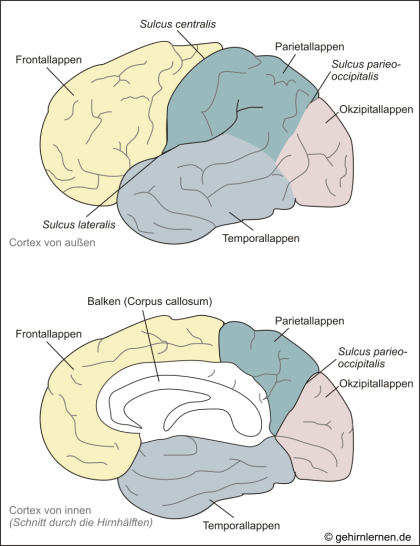
\includegraphics[width=0.8\linewidth]{grafiken/abb3.png}
\caption{Gliederung des Cortex\\ Quelle:  \cite{Schaefers.2014}}
\label{fig:Gehirn3}
\end{figure}

\subsubsection{Das limbische System}
Das limbische System ist die Zusammenfassung mehrerer Strukturen zu einem funktionellen System. Dazu gehören die Strukturen am \glqq Übergang von Cortex (bewusste Vorgänge, Wahrnehmungen) und dem Zwischenhirn (Nicht-bewusste Vorgänge und Wahrnehmungen).\grqq \citep[S. 36]{Derouiche.2011} Es umfasst u. a. den Hippocampus, die Amygdala und den Nucleus Accumbens. Nach \citet[S. 270]{Kirschbaum.2008} ist es das  \glqq Zentrum der Emotion, der Motivation und des Lernens im menschlichen Gehirn.\grqq 
\newline Der Hippocampus ist neben der räumlichen Orientierung auch für das deklarative Gedächtnis zuständig. Es kann also zugeordnet werden, ob eine Situation neu oder bereits bekannt ist. \citep[S. 36]{Derouiche.2011} Durch die Aktivierung der Amygdala werden Wut, Angst und Ekel ausgelöst. Durch die Verbindung zum Hypothalamus im Zwischenhirn, der Steuerungszentrale des vegetativen Nervensystems, kann die Amygdala u.a. einen erhöhten Herzschlag, Blutdruck und Schweißausbruch auslösen. \citep[S. 36f]{Derouiche.2011} Die Amygdala ist für das \glqq emotionale Färben von Informationen\grqq zuständig. \citep[S. 12]{Kirschbaum.2008} Das bedeutet, dass die Amygdala z.B. Situationen oder Orte durch \glqq emotionales Lernen\grqq mit einer Emotion wie Angst verknüpfen kann. Das führt z.B. dazu, dass durch dieses \glqq emotionale Gedächtnis\grqq ein Ort oder Situation mit einer Emotion wie Angst verknüpft werden kann. \citep[S. 37]{Derouiche.2011}    
\newline Der Nucleus accumbens reagiert auf positive, lustvermittelnde Reize. Er wird durch Dopamin aktiviert, steuert die Freisetzung von Endorphinen, was zu einem Glückgsgefühl führt. \glqq Eine verminderte Dopaminfreisetzung (…) kann zum Verlust jeglicher Motivation führen.\grqq \citep[S. 11]{Nowka.2013}

\subsubsection{Mesolimbisches Dopaminsystem}
Das mesolimbische Dopaminsystem ist ein bedeutender Teil des Belohnungssystems im Gehirn, da es unter anderem Zentrum der Dopaminausschüttung ist. Es  reicht vom Nucleus Accumbens bis zum Cortex und hat seinen Urpsrung im ventralen tegmentalen Areal (VTA). \citep[S. 11]{Nowka.2013} Die Aktivierung löst \glqq Empfindungen und Verhalten wie Wohlempfinden, erotisches Empfinden, \glqq incentive behaviour\grqq, Appetenzverhalten und Sucht\grqq aus. \cite[S. 37]{Derouiche.2011} 
\newline Ein Reiz löst im VTA eine Dopaminausschüttung beim Nucleus Accumbens aus. Die Menge des Dopamins ist ein Maß dafür, wie sehr etwas gewollt wird, nicht ob es wirklich gemocht wird. Das Dopamin dockt dann am präfrontalen Cortex an, wo das Bewusstsein liegt. Dort wird dann eine Entscheidung gefällt. Nach der Befriedigung des Bedürfnisses meldet die Großhirnrinde ein positives Erlebnis ans VTA. Danach erfolgt eine Serotoninausschüttung, die beruhigend und befriedigend wirkt. \cite[S. 16]{Seelbach.2011}

\subsection{Bildgebende Messmethoden}
Das Gebiet der Psychophysiologie umfasst die noninvasive Erforschung der Zusammenhänge zwischen psychologischen Prozessen und der physiologischen Aktivitäten. Zu den ersten Messverfahren rein elektrophysiologische Verfahren. In den letzten Jahren kommen vermehrt bildgebende Verfahren zum Einsatz. \citep[S. 232]{Kirschbaum.2008}
Die Entwicklung dieser bildgebender Messmethoden lässt eine detaillierte Analyse der Wirkung von Anreizen und die ablaufenden Prozesse im Gehirn  zu. Mit Hilfe dieser dieser neuen Möglichkeiten konnten und können neue neurowissenschaftliche Erkenntnisse und Zusammenhänge erforscht werden. \citep[S. 15]{Nowka.2013}
 
Messungen mit Hilfe der Elektroenzephalographie (EEG) waren die ersten, welche es ermöglichten das Gehirn in vivo zu untersuchen. \citep[S. 43]{Weber.2011}  Die Magnetresonanz-Enzephalographie (MEG), die Positronen-Emissions-Tomographie (PET)  und die funktionelle Magnetresonanztomographie (fMRT) sind die modernen bildgebenden Verfahren, wobei die fMRT die zurzeit beste Methode ist, emotionale Reaktionen und kognitive Leistungen im Gehirn zu untersuchen. \citep[S. 50]{Weber.2011}
 
Mit Hilfe des aktuellen Forschungsstandes und den \glqq Messmethoden können Anreize anhand ihrer neurobiologischen Wirkung bewertet und verbessert werden.\grqq \citep[S. 17]{Nowka.2013}